\section{Discussion}
\label{sec:discussion}

We have considered two ways to evaluate the performance of our approach: computing the average distance from the test fit to the ground truth data and visually analyzing the  test or target fit on the CT image. 

%% --------------------------------------------

\subsection{Likelihood Evaluators}
\label{subsec:evaluators}

Applying multiple Markov chains in sequence was the attempt at a solution to a problem faced early in the project.
While very strong at precise fits, ASM struggled with general alignment to the CT image on a larger scale: It would align the model to the nearest occurrences of tissue, even if that was not the corresponding part of the bone contour.
To avoid this local optimum, we introduced the leading Markov chain using landmark correspondence in the likelihood evaluator.
This would get the model to align roughly to the bone contour. 

After that, we would follow up with the active shape model evaluator which should then closely fit the model to the contours. 
This approach worked very well. 
The landmark evaluator helped to avoid or break out of local minima while the active shape model helped to get a very close fit.

Both our evaluators are product evaluators including the prior probability either with the landmarks' fit or the profiles.
We also tried adding the landmarks' evaluator to the product for the second and third chain.
However, this did not lead to any improvement in our result and the change was hence discarded from the final configuration.

%% --------------------------------------------

\subsection{Proposals}
\label{subsec:proposals}

The plan for our proposals was to expand on the idea of multiple sequential Markov chains explained in Section~\ref{subsec:evaluators}: Some of the proposals are more useful during a fitting process on a larger scale while some are better suited for fitting on a small scale. 
We tested a number of different configurations for the parameters involved in the proposals, \ie, the combination of different proposals with different standard deviations. 
The configuration shown in Section~\ref{sec:results} provided the best results among all of our experiments. 

Generally, it is sensible to use larger standard deviations early on and set them to continually smaller values.
This way, we take larger steps in the beginning and go on fitting details of the shape towards the end.

Furthermore, we put a larger emphasis on rotation and translation during the first chain and gradually shifted the focus to shape transformations.

%% --------------------------------------------

\subsection{Test Fit}
\label{subsec:testfit}

The average distance of 0.56 millimeters for our test fits is a satisfying result.
We considered this difference to the ground truth to be reasonably small, leading to the conclusion that the procedure works reliably overall. 

When looking at the meshes, we see that the model sometimes gets stuck in a local minimum.
This risk is especially high at parts of the CT image where an adjacent bone is particularly close to the femur. 
On the left hand side of \autoref{fig:testfit} we see an example where the algorithm converges the true shape, but it is evident that small variations can move the femur head towards the contour of the pelvis.
The right hand side shows the same fit a few slices further on top of the femur head, where the model got stuck in the contour of this adjacent bone.
Further optimization would be necessary to escape such local optima consistently.

\begin{figure}
	\centering
  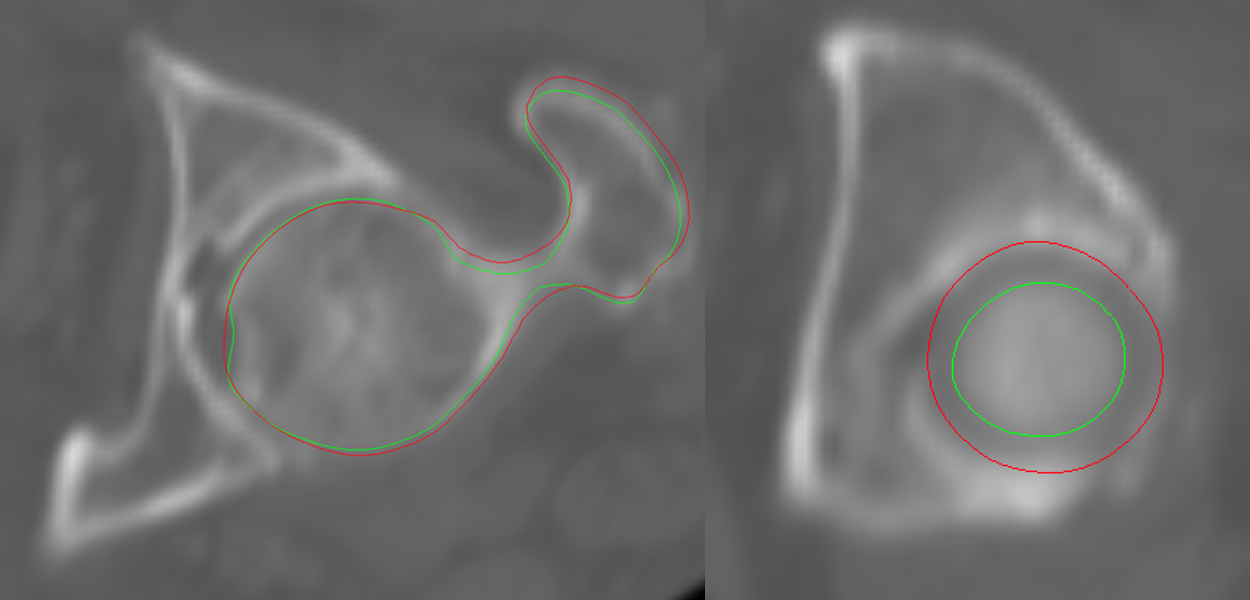
\includegraphics[width=\columnwidth]{./Figures/local_minimum_comparison}
  \caption{
    Two cuts through the image, the fitted model (red) and the ground truth mesh (green).
    On the left, the model successfully escaped the local minimum.
    On the right, it got stuck in a local minimum.
  }
  \label{fig:testfit}
\end{figure}

%% --------------------------------------------

\subsection{Target Fit}
\label{subsec:targetfit}

\todoQuestion{Maybe remove? In my opinion, this does not contribute much to the discussion.}
\autoref{fig:targetfit} shows that the procedure appears to be working for the target CT images as well, as the model is tightly fit to the image contours. An option we considered was to increase the landmark noise variance for this part as we could not double check clicked landmarks on the ground truth mesh, but ultimately, this did not seem necessary due to the many iterations of the procedure afterwards.

\begin{figure}
	\centering
  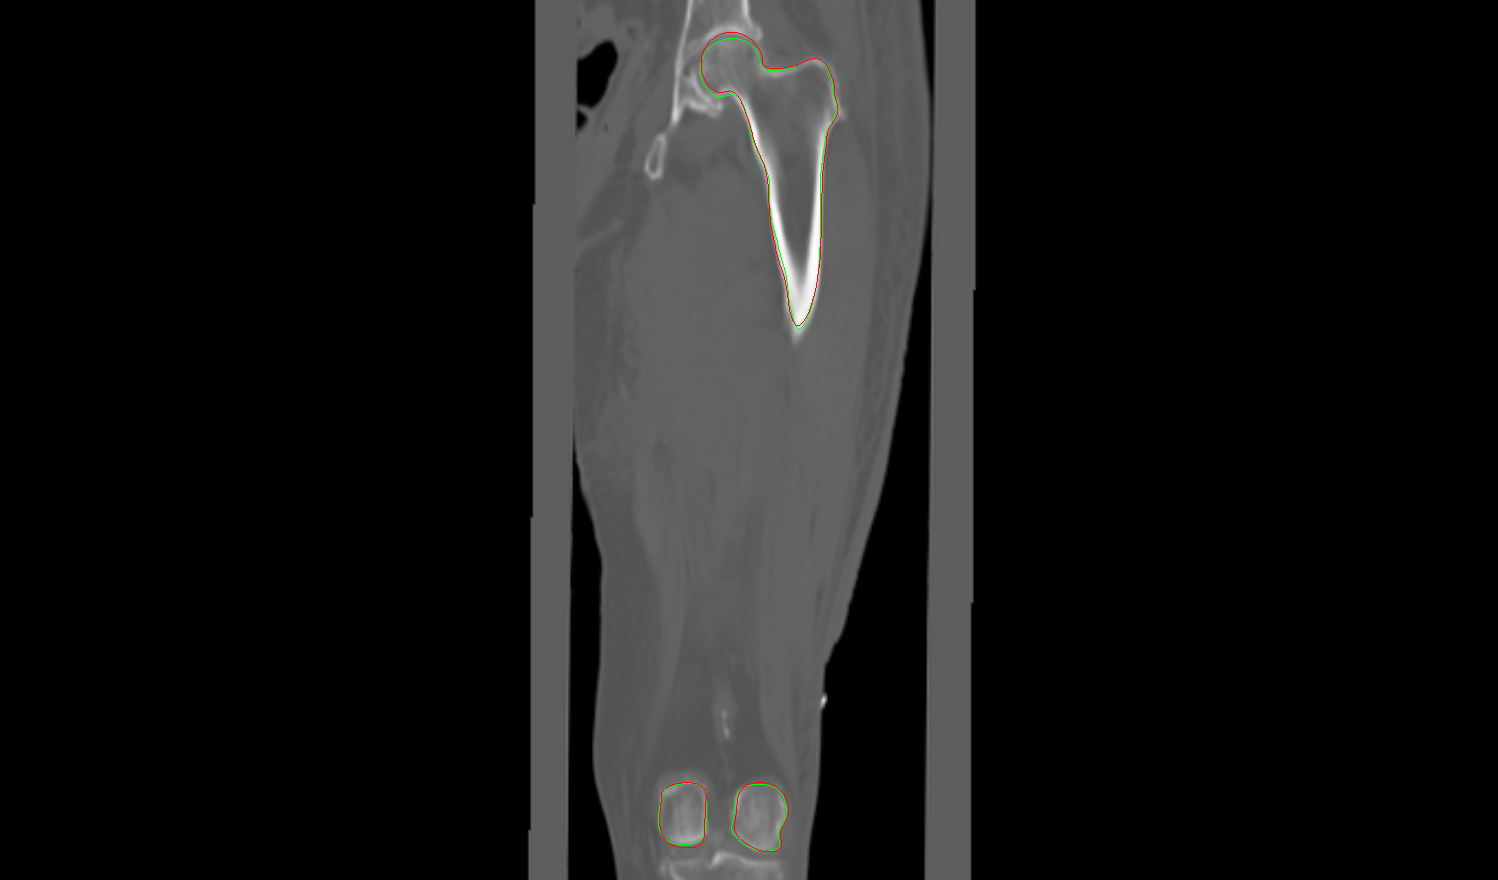
\includegraphics[width=\columnwidth]{./Figures/local_minimum_y-axis}
  \caption{
    Example of a fit of our model to the target CT image. }
  \label{fig:targetfit}
\end{figure}
\todoRevise{Figure with target fit}




